\section{Themenmodelle}
\label{sec:topicModels}

Ein Themenmodell \citep{Hofmann1999,Blei2003LDA,Steyvers2006} ist ein statistisches Modell um Themen aus Textkorpora zu extrahieren. Dazu werden Terme gruppiert, die oft zusammen auftreten. Diese Gruppierung wird als Thema bezeichnet. Ein Thema ist demnach durch die Verteilung der zugehörigen Terme charakterisiert. Ein Term kann dabei zu mehreren Themen gehören. 

Die  Themen werden mit den zwei Termen, die mit der höchsten Wahrscheinlichkeit zu einem Thema gehören, benannt. Die beiden Themen in Abbildung \ref{fig:tmGenerator} würden mit \textit{film regisseur} und \textit{erdbeben richterskale} bezeichnet. So kann in mehr oder weniger direkt auf den Inhalt des Themas geschlossen werden und die Themenbezeichnung ist besser lesbar.  

Um die Themen aus dem Textkorpus zu extrahieren, wird ausgehend von einem generativen Modell eine Methode zur Inferenz der Themen aus den beobachteten Wörtern entwickelt. 
\begin{figure}[ht]
  \centering
  \subfigure[Generativer Prozess]{
    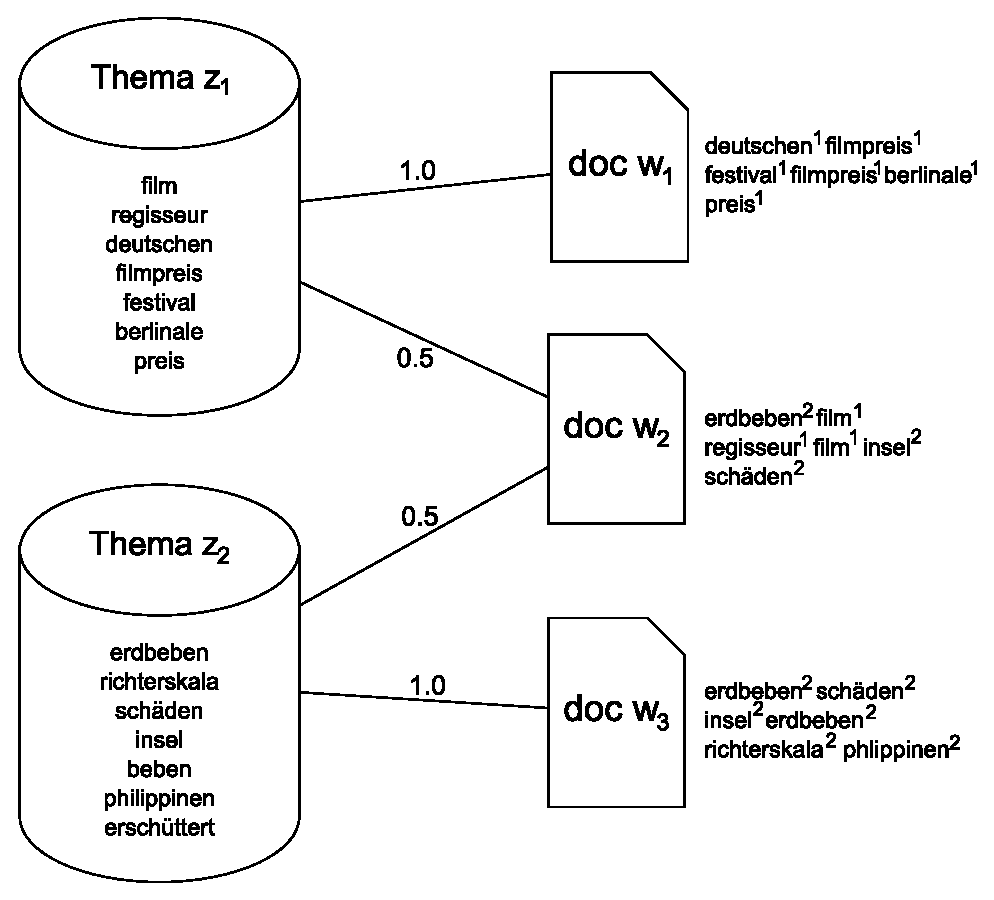
\includegraphics[scale=0.4]{images/content/02_fundamentals/topicModelGenerater}
    \label{fig:tmGenerator}
  }
  \subfigure[Statistische Inferenz]{
    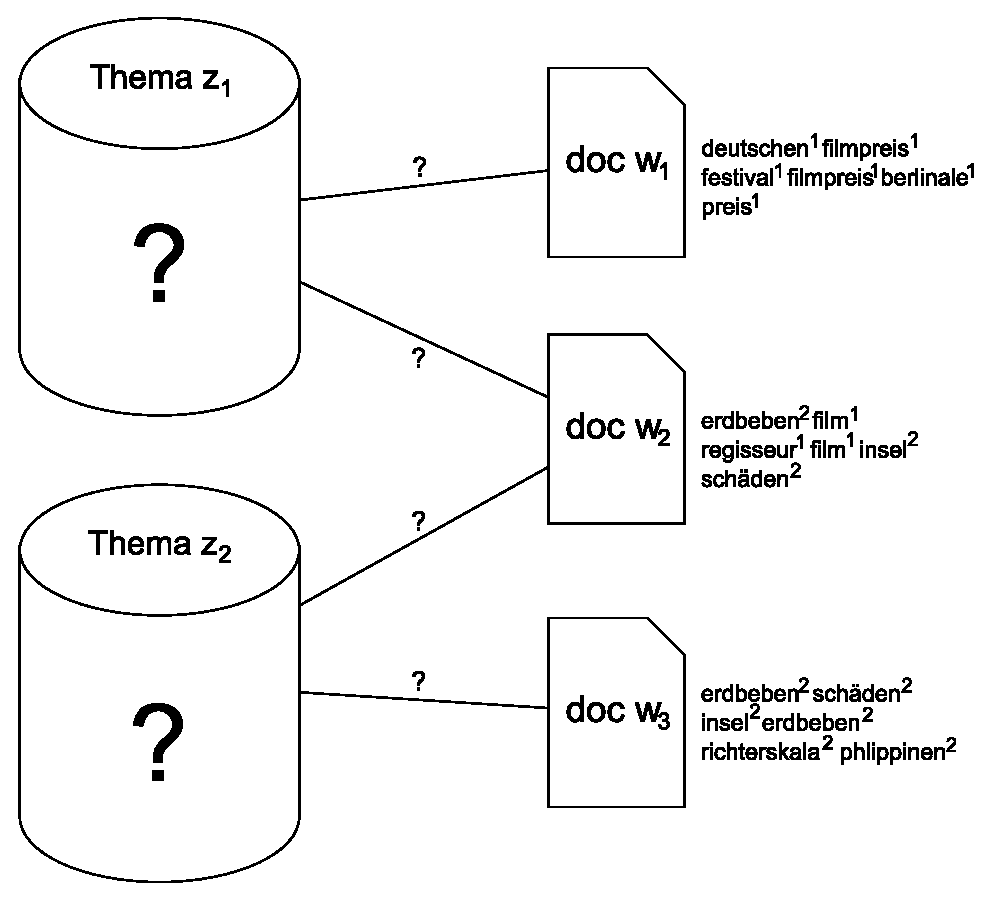
\includegraphics[scale=0.4]{images/content/02_fundamentals/topicModelStatInf}
    \label{fig:tmStatInf}
  }
\caption{Problemstellung der Themen Modelle nach \citep{Steyvers2006}.}
\end{figure}

Der generative Prozess beschreibt, wie aus Themen und den zugehörigen Termen Dokumente generiert werden. Dazu fassen Themenmodelle die Dokumente als Mischung verschiedener Themen auf. Für jedes Dokument wird eine Wahrscheinlichkeit festgelegt, mit der dieses Dokument zu einem Thema gehört. Anhand dieser Wahrscheinlichkeit wird für jedes Wort in einem Dokument ein Term aus dem Thema gezogen. In Abbildung \ref{fig:tmGenerator} wird dieser Prozess schematisch dargestellt. 

Hier werden zwei Themen dargestellt, einmal ein Thema über Filme und ein Thema über Erdbeben. Für Dokument $\doc_1$ und $\doc_3$ wurde jeweils festgelegt, dass sie nur aus Thema $\docTopic_1$ bzw. $\docTopic_2$ bestehen. Dementsprechend werden Wörter nur aus den Termen des zugehörigen Themas gezogen. Dokument $\doc_2$ besteht jeweils zur Hälfte aus Thema $\docTopic_1$ und $\docTopic_2$. Es werden also Terme aus beiden Themen gezogen. Für jedes Wort wird vorher ermittelt, aus welchem Thema ein Term gezogen werden soll. Anschließend wird aus dem so bestimmten Thema ein Term gezogen. So kann ein Dokument generiert werden, das sowohl das Thema Film als auch Erdbeben beinhaltet. Die so generierten Dokumente weisen keine syntaktische Struktur auf, da vom generativen Prozess keine vollständigen Sätze erzeugt werden. Die Wörter instantiieren nur Terme aus den Themen. Dafür sind die Wahrscheinlichkeiten der Themen in diesem Dokument bekannt.

Das generative Modell erlaubt es zwar Dokumente zu bestimmten Themen zu erzeugen, die eigentliche Zielsetzung ist jedoch, für ein Textkorpus Themen zu identifizieren. Die Abbildung \ref{fig:tmStatInf} zeigt analog zu Abbildung \ref{fig:tmGenerator} das Problem auf: Aus Wörtern, die in Dokumenten beobachtet wurden, sollen Themen abgeleitet werden. 
Aus dem generativen Modell kann man mit statistischen Mitteln eine Methode entwickeln, die es erlaubt, aus den beobachteten Daten das dazu passende Modell zu finden. Im folgenden wird anhand der Latent Dirichlet Allocation (LDA) diese Methode hergeleitet. 

\subsection{Latent Dirichlet Allocation}

Der Algorithmus Latent Dirichlet Allocation (LDA) gibt ein probabilistisches Modell zur Erzeugung von Dokumenten an. Anhand dieses Modells kann eine Methode zur statistischen Inferenz von Themen aus beobachteten Wörtern entwickelt werden. In Abbildung \ref{fig:ldaModel} wird das generative Modell als graphisch dargestellt. Im Unterschied zu anderen Themenmodellen gibt die LDA zusätzlich zur Termverteilung von Themen noch eine Themenverteilung für Dokumente an \citep{Hofmann1999}. 

\begin{figure}[ht]
  \centering
  \begin{pspicture}(0,-0.5)(4,6)

\pscircle[fillstyle=solid, fillcolor=grey](2,1){0.5} 
\rput(1.1,1){$w_{m,n}$}
\pscircle(2,3){0.5} 
\rput(1.1,3){$z_{m,n}$}
\pscircle(2,5){0.5} 
\rput(1.1,5){$\vartheta_{m}$}
\psline{<-}(2,1.5)(2,2.5)
\psline{<-}(2,3.5)(2,4.5)

\pscircle(4.5,5){0.5}
\psline{<-}(2.5,5)(4,5)
\rput(4.5,4.25){$\alpha$}

\pscircle(4.5,1){0.5}
\psline{<-}(2.5,1)(4,1)
\rput(4.5,1.75){$\varphi_{k}$}

\pscircle(6.5,1){0.5}
\psline{<-}(5,1)(6,1)
\rput(6.5,1.75){$\beta$}

\psframe(0.2,-0.5)(3.5,6)
\rput(3.2,-0.2){$M$}

\psframe(0.6,0.3)(3.2,4.0)
\rput(2.9,0.6){$N$}

\psframe(3.75,0.25)(5.5,2.0)
\rput(5.2,0.5){$K$}

\end{pspicture}
  \caption{Generatives Modell für LDA nach \citep{Blei2003LDA}.}
  \label{fig:ldaModel}
\end{figure}

In Abbildung \ref{fig:ldaModel} wird dargestellt, wie ein Dokument erzeugt wird. Die Pfeile geben Abhängig"-keiten zwischen den Variablen an, während die Kacheln Wiederholungen von Variablen anzeigen. Die Buchstaben in den Kacheln geben an, wie oft die Variablen wiederholt werden. So können die Knoten für $M$ Dokumente und $M \times N$ Wörter präziser dargestellt werden ohne die Variablen mehrfach zu notieren. Der schattierte Knoten gibt an, dass diese Variable beobachtbar ist und die leeren Knoten zeigen latente Variablen an. 

Für jedes Dokument $\doc_m$, wird eine Themenverteilung $\docTopicDist{m}$ ermittelt. Anhand dieser wird für jedes Wort $\word_{m,n}$ aus Dokument $\doc_m$ ein Thema $\wordTopic_{m,n}=k$ gezogen. Aus der Termverteilung $\topicTermDist{k}$ für das Thema $\wordTopic_{m,n}=k$ wird nun der Term bestimmt, der das Wort instantiiert. 

Die Parameter $\alpha$ und $\beta$ sind die Parameter der Dirichletverteilung, anhand derer die multinomialen Themenverteilungen $\docTopicDist{m}$ und die Termverteilungen $\topicTermDist{k}$ bestimmt werden. Im Weiteren wird $\alpha$ bzw. $\beta$ synonym für $\alpha := (\alpha_1,\ldots,\alpha_k)$ und die symmetrische Variante $\alpha := \alpha_1 = \ldots = \alpha_k$ benutzt. Die Menge aller Themenverteilungen $\docTopicDist{m}$ wird als $\Theta = \left\{\docTopicDist{m}\right\}^M_{m=1}$ bezeichnet und die Menge aller Wortverteilungen $\topicTermDist{k}$ als $\Phi = \left\{\topicTermDist{k}\right\}^K_{k=1}$. 

Aus dem generativen Modell können nun verschiedene Wahrscheinlichkeiten abgeleitet werden. So ist die Wahrscheinlichkeit, dass ein Wort $w_{m,n}$ einen Term $t$ instantiiert, gegeben eine Themenverteilung $\docTopicDist{m}$ für das Dokument $m$
\begin{equation}
  p(\word_{m,n}=t|\docTopicDist{m},\Phi) = \sum^K_{k=1} p(\word_{m,n}=t|\topicTermDist{k})p(\wordTopic_{m,n}=k|  \docTopicDist{m})
\label{eq:ldaWordProbabilty}
\end{equation}
Dies entspricht einer Iteration der Wortkachel, die die Knoten $\wordTopic_{m,n}$ und $word_{m,n}$ enthält. Die gemeinsame Wahrscheinlichkeitsverteilung für alle beobachteten und unbeobachteten Variablen kann anhand des Modells in Abbildung \ref{fig:ldaModel} abgeleitet werden. 
\begin{equation}
p(\doc_m,\docTopic_m,\docTopicDist{m},\Phi|\alpha,\beta) = \overbrace{\underbrace{\prod^{N_m}_{n=1}p(w_{m,n}|\topicTermDist{\wordTopic_{m,n}})p(\wordTopic_{m,n}|\docTopicDist{m})}_{\text{Wortkachel}} \cdot p(\docTopicDist{m}|\alpha)}^{\text{Dokumentkachel (nur 1 Dokument)}} \cdot \underbrace{p(\Phi|\beta)}_{\text{Themenkachel}}
\label{eq:ldaDocJointDistribution}
\end{equation}

Integriert man nun über $\docTopicDist{m}$ und $\Phi$ und summiert über alle Themen $\wordTopic_{m,n}$ erhält man mit (\ref{eq:ldaWordProbabilty}), die Wahrscheinlichkeit für ein Dokument $\doc_m$.

\begin{align}
p(\doc_m|\alpha,\beta) &= \int \int p(\docTopicDist{m}|\alpha)p(\Phi|\beta)\cdot \prod^{N_m}_{n=1} \sum_{\wordTopic_{m,n}} p(\word_{m,n}|\topicTermDist{\wordTopic_{m,n}})p(\wordTopic_{m,n}|\docTopicDist{m})d\Phi d\docTopicDist{m} \\ &=  \int \int p(\docTopicDist{m}|\alpha)p(\Phi|\beta)\cdot \prod^{N_m}_{n=1} p(\word_{m,n}|\docTopicDist{m},\Phi)d\Phi d\docTopicDist{m}
\label{eq:ldaDocDistribution} 
\end{align}

Die Wahrscheinlichkeit für ein komplettes Korpus erhält man, indem man $M$ mal ein Dokument erzeugt. Die Wahrscheinlichkeit für ein Korpus kann also mit folgender Formel ausgedrückt werden.

\begin{equation}
p(\corpus|\alpha,\beta) = \prod^M_{m=1} p(\doc_m|\alpha,\beta)
\end{equation}

\subsection{Inferenz mit Gibbs-Sampling}

Man kann nun ausgehend von diesen Wahrscheinlichkeiten eine Methode zur Inferenz der unbeobachteten Themen entwickeln. Hierzu nutzt man einen approximativen Algorithmus, da trotz der relativen Einfachheit des Modells eine exakte Inferenz nicht möglich ist. Hier benutzen wir dazu Gibbs-Sampling \citep{Walsh2004} . 

Gibbs-Sampling ist eine Monte Carlo Markov Ketten (MCMC) Simulation. Mit MCMC Methoden kann man hochdimensionale  Wahrscheinlichkeitsverteilungen anhand einer Markov Kette simulieren. Dies erlaubt es, die gesuchte Verteilung $p(\docTopic|\doc)$, welche Themen in welchen Dokumenten auftreten, zu berechnen. Mit exakter Inferenz ist diese Verteilung sehr schwierig zu berechnen \citep{parameterEstimation}. Der Gibbs-Sampling Algorithmus berechnet die Verteilung nicht exakt sondern nähert die Verteilung an. Der Algorithmus funktioniert wie folgt.

Sei $p(w,z)$ eine bivariate Zufallsvariable. Wir wollen $p(z)$ bzw. $p(w)$ berechnen. Anstatt nun $\int p(w,z)dw$ bzw. $\int p(w,z)dz$ direkt zu berechnen, berechnet der Gibbs-Sampler alternierende Sequenzen von $p(w|z)$ und $p(z|w)$. Das Sampling wird mit einem zufälligen Wert für $z_0$ gestartet und sampelt $w_0$ anhand $p(w|z=z_0)$. Dann wird $w_0$ dazu benutzt $z_1$ anhand der bedingten Verteilung $p(z|w=w_0)$ zu ermitteln. Das Sampling wird dann nach folgender Formel fortgesetzt:
\begin{align*}
w_i & \approx p(w|z=z_{i-1})  \\
z_i & \approx p(z|w=w_{i})
\end{align*}
Nach $k$-maliger Wiederholung konvergiert die Sequenz gegen die tatsächliche Verteilung. 

Für den multivariaten Fall wird die bedingte Wahrscheinlichkeit erweitert, indem aus dem Variablenvektor $\mathbf{w}$ die $k$-te Variable aus der Verteilung $p(w_i|\mathbf{w}_{\neg i})$ gezogen wird. Wobei $\mathbf{w}_{\neg i} = (w_1,\ldots,w_{i-1},w_{i+1},\ldots,w_k)$ ist. 

Für die LDA wollen wir nun die Verteilung $p(\docTopic|\doc)$ abschätzen. Um dies berechnen zu können, müssen wir die gemeinsame Verteilung $p(\docTopic,\doc)$ bzw. $p(\doc)$ kennen (siehe Gleichung \ref{eq:gibbsLDA})

\begin{align}
p(\docTopic|\doc) = \frac{p(\doc,\docTopic)}{p(\doc)} = \frac{\prod^W_{i=1}p(\word_i|\wordTopic_i)}{\prod^W_{i=1}\sum^K_{k=1}p(\wordTopic_i=k,\word_i)}
\label{eq:gibbsLDA}
\end{align}

Hier hilft uns die Gibbs-Sampling Prozedur, die es erlaubt, $p(\docTopic|\doc)$ direkt zu berechnen, ohne über $K^W$ Terme zu summieren. Der Gibbs-Sampler simuliert die Verteilung $p(\docTopic|\doc)$ durch 
\begin{equation}
p(\wordTopic_i|\docTopic_{\neg i }, \doc) = \frac{p(\doc,\docTopic)}{p(\docTopic_{\neg i},\doc)} 
\end{equation}

Hierzu müssen wir die gemeinsame Verteilung $p(\doc,\docTopic)$ kennen. Im Falle der LDA kann diese Verteilung aufgespalten werden in 
\begin{equation}
p(\doc,\docTopic|\alpha,\beta) = p(\doc|\docTopic,\beta)\cdot p(\docTopic|\alpha)\text{,}
\end{equation}
da $\doc$ unabhängig von $\alpha$ ist und $\docTopic$ unabhängig von $\beta$.

Die Faktoren können einzeln hergeleitet werden. So ist 
\begin{align}
p(\doc|\docTopic,\beta) &= \int p(\doc|\docTopic,\Phi) p(\Phi|\beta) d\Phi \notag \\
                        &= \int \prod^K_{z=1}\frac{1}{\Delta(\beta)} \prod^V_{t=1}\topicTermProb{z}{t}^{n^{(t)}_z+\beta_t-1} d\topicTermDist{z} \label{eq:ldaGibbsIntegral1}\\
                        &= \prod^K_{z=1}\frac{\Delta(\mathbf{n}_z+\beta)}{\Delta(\beta)}, \ \ \mathbf{n}_z=\left\lbrace n_z^{(t)}\right\rbrace^V_{t=1} \label{eq:ldaGibbsIntegral2}
\end{align}

Hier wird benutzt, dass $p(\doc|\docTopic,\Phi)$ multinomial und $p(\Phi|\beta)$ dirichlet verteilt ist. Unter der Annahme, dass die Reihenfolge der Wörter in einem Dokument unerheblich ist, gilt:
\begin{align*}
p(\doc|\docTopic,\Phi) %&= \prod^W_{i=1}p(\word_i|\wordTopic_i) = \prod^W_{i=1}\topicTermProb{z_i}{w_i} \\
					   &= \prod^K_{k=1}\prod_{i:z_i=k}p(\word_i=t|\wordTopic_i=k) = \prod^K_{k=1}\prod^V_{t=1}\topicTermProb{k}{t}^{n^{(t)}_k}
\end{align*}
und 
\begin{align*}
Dir(\topicTermDist{k}|\beta) = \frac{1}{\Delta(\beta)}\prod^V_{t=1} \topicTermProb{k}{t}^{\beta_{t}-1} \text{ mit } \Delta(\beta)=\frac{\prod^{dim \beta}_{k=1}\Gamma(\beta_k)}{\Gamma(\sum^{dim \beta}_{k=1}\beta_k)}
\end{align*}
Aus den beiden vorhergehenden Gleichungen ergibt sich \ref{eq:ldaGibbsIntegral1}. Die Anwendung des Dirichletintegrals auf Gleichung \ref{eq:ldaGibbsIntegral1} ergibt dann Gleichung \ref{eq:ldaGibbsIntegral2}.

Analog kann $p(\docTopic|\beta)$ hergeleitet werden. Es ist:
\begin{align}
p(\docTopic|\alpha) &= \int p(\docTopic|\Theta) p(\Theta|\alpha) d\Theta \notag\\
                    &= \int \prod^M_{m=1}\frac{1}{\Delta(\alpha)}\prod^K_{k=1}\docTopicProb{m}{k}^{n^{(k)}_m + \alpha_k-1}  d\docTopicDist{m} \\
                    &= \prod^M_{m=1} \frac{\Delta(\mathbf{n}_m+\alpha)}{\Delta(\alpha)}, \ \ \mathbf{n}_m=\left\lbrace n_m^{(k)}\right\rbrace^K_{k=1} \label{eq:ldaPZ}
\end{align}

Die gemeinsame Verteilung $p(\doc,\docTopic|\alpha,\beta)$ ergibt sich aus \ref{eq:ldaPZ} und \ref{eq:ldaGibbsIntegral2}. 
\[
p(\doc,\docTopic|\alpha,\beta) = \prod^K_{z=1}\frac{\Delta(\mathbf{n}_z+\beta)}{\Delta(\beta)} \cdot \prod^M_{m=1} \frac{\Delta(\mathbf{n}_m+\alpha)}{\Delta(\alpha)}
\]

Wenn man nun die gemeinsame Verteilung einsetzt, ergibt sich die Update-Gleichung für den Gibbs-Sampler. 

\begin{align}
p(\wordTopic_i=k|\docTopic_{\neg i},\doc) &= \frac{p(\doc,\docTopic)}{p(\doc,\docTopic_{\neg i})} = \frac{p(\doc,\docTopic)}{p(\doc_{\neg i},\docTopic_{\neg i})p(\word_i)} \frac{p(\docTopic)}{p(\docTopic_{\neg i})} \\
&\propto \frac{\Delta(\mathbf{n}_z+\beta)}{\Delta(\mathbf{n}_{z,\neg i} + \beta)} \cdot \frac{\Delta(\mathbf{n}_m+\alpha)}{\Delta(\mathbf{n}_{m.\neg i} + \alpha)} \\
&\propto \ldots \notag \\
&\propto \frac{n^{(t)}_{k,\neg i}+\beta}{\sum^{V}_{t=1}n^{(t)}_{k,\neg i} + \beta} \cdot \frac{n^{(k)}_{m,\neg i}+\alpha}{\sum^{K}_{k=1}n^{(k)}_{m,\neg i} + \alpha} \label{eq:updateEqSeen}
\end{align} 

Die Update-Gleichung kann nun dazu benutzt werden, die Themen für Wörter in Dokumenten zu bestimmen. Es wird über alle Wörter in den Dokumenten iteriert und für jedes Wort anhand $p(\wordTopic_i=k|\docTopic_{\neg i},\doc)$ ein neues Thema bestimmt. Dies wird solange wiederholt, bis die Themenverteilung stabil bleibt, bzw. der Gibbs-Sampler einen stabilen Zustand erreicht hat. Die Verteilungen $\docTopicDist{m}$ und $\topicTermDist{k}$ können direkt aus den Gleichungen \ref{eq:ldaGibbsIntegral2} und \ref{eq:ldaPZ} abgeleitet werden. So hat man nun ein Modell, welches Dokumente bzw. Wörter in Themen gruppieren kann. Genaueres zur Herleitung und Gibbs-Sampling im Kontext der LDA kann in \citep{Griffiths2004LDA} nachgelesen werden.

\subsection{Inferenz für ungesehene Dokumente}
\label{subsec:infUnseen}

Ausgehend vom gelernten Modell will man nun für neue Dokumente die Themen herausfinden. Sei $\tilde{\doc}$ ein neues Dokument. Für dieses neue Dokument lassen wir wiederum den Gibbs-Sampler die Themen bestimmen. Anstatt $p(\wordTopic_i=k|\docTopic_{\neg i},\doc)$ bestimmen wir aber $p(\tilde{\wordTopic}_i=k|\tilde{\docTopic}_{\neg i},\tilde{\doc},\Phi,\Theta)$, da wir die Themen für das neue Dokument anhand der schon ermittelten Themen- und Termverteilungen inferieren wollen. Es ergibt sich folgende Update-Gleichung
\begin{equation}
p(\tilde{\wordTopic}_i=k|\tilde{\docTopic}_{\neg i},\tilde{\doc},\Phi,\Theta) = \frac{n^{(t)}_{k}+\tilde{n}^{(t)}_{k, \neg i}+\beta}{\sum^V_{t=1}n^{(t)}_{k}+\tilde{n}^{(t)}_{k, \neg i}+\beta}\cdot \frac{n^{(k)}_{\tilde{m},\neg i}+\alpha}{\sum^K_{k=1}n^{(k)}_{\tilde{m},\neg i}+\alpha} 
\label{eq:updateEqUnseen}
\end{equation}
wobei $\tilde{n}^{(t)}_{k}$ die Anzahl des Auftreten von Term $t$ mit Thema $k$ für das neue Dokument $\tilde{\doc}$ bezeichnet. Analog zu normaler Inferenz können auch hier die Dokumentverteilung $\docTopicDist{m}$ und die Termverteilung $\topicTermDist{k}$ bestimmt werden. So können für ein neues Dokument die vorherrschenden Themen bestimmt werden. 

Ein Problem sind Terme, die vorher nicht aufgetreten sind. Diese erscheinen in den Termverteilungen der Themen nicht und können somit nicht dazu beitragen, Themen zu inferieren. Sie fließen somit auch nicht in die Updategleichung \ref{eq:updateEqUnseen} mit ein. Im Falle der Inferenz werden sie einfach übersprungen.


